\chapter{An introduction to \texttt{R}}
\label{ch:R}

\texttt{R} is an increasingly popular programming language that is
available free of charge on any operating system at
\href{https://r-project.org}{\tt https://r-project.org}. A number of
different graphical user interfaces (GUIs) are available for
\texttt{R}, the most popular of which are \texttt{RGui},
\texttt{RStudio}, \texttt{RCommander} and \texttt{Tinn-R}.  For this
tutorial, however, the simple command line console suffices. This
chapter introduces all the functions that are needed to solve the
exercises in Chapter~\ref{ch:exercises}. A more complete listing of
base \texttt{R} functions is provided at
\href{https://cran.r-project.org/doc/contrib/Short-refcard.pdf} {\tt
  https://cran.r-project.org/doc/contrib/Short-refcard.pdf}.

\section{The basics}
\label{sec:R-basics}

\begin{enumerate}
\item We will start this tutorial from the \texttt{R} \textbf{command
  prompt}, which is the window that begins with a \verb|>|
  symbol. First, do some arithmetic:

\begin{console}
> 1 + 1
[1] 2
\end{console}

\texttt{R} prints the result to the command prompt (\verb|2| in this
case). Here are some other arithmetic operations:

\begin{console}
> sqrt(2)
[1] 1.414214
> exp(log(10))
[1] 10
> 13%%5
[1] 3
\end{console}

\item An arrow operator is used to assign a value to a variable. Note
  that the arrow can point both ways:

\begin{console}
> foo <- 2
> 4 -> bar
> foo <- foo*bar
> foo
[1] 8
\end{console}

\item Create a vector of numbers:

\begin{console}
> myvec <- c(2,4,6,8)
> myvec*2
[1]  4  8 12 16
\end{console}

Query the third value of the vector:

\begin{console}
> myvec[3]
[1] 6
\end{console}

Change the third value of the vector:

\begin{console}
> myvec[3] <- 100
\end{console}

Change the second and the third value of the vector:

\begin{console}
> myvec[c(2,3)] <- c(100,101)
\end{console}

Create a sequence of numbers:

\begin{console}
> seq(from=1,to=10,by=1)
 [1]  1  2  3  4  5  6  7  8  9 10
\end{console}

Equivalently (output omitted for brevity):

\begin{console}
> seq(1,10,1)
> seq(1,10)
> seq(to=10,by=1,from=1)
> seq(to=10)
> 1:10
\end{console}

Create a 10-element vector of twos:

\begin{console}
> rep(2,10)
 [1] 2 2 2 2 2 2 2 2 2 2
\end{console}

\item Create a 2 $\times$ 4 matrix of ones:

\begin{console}
> mymat <- matrix(1,nrow=2,ncol=4)
\end{console}

Change the third value in the first row of \texttt{mymat} to 3:

\begin{console}
> mymat[1,3] <- 3
\end{console}

Change the entire second column of \texttt{mymat} to 2:

\begin{console}
> mymat[,2] <- 2
\end{console}

Remove the first column from \texttt{mymat}:

\begin{console}
> mymat[,-1]
     [,1] [,2] [,3]
[1,]    2    3    1
[2,]    2    1    1
\end{console}

Give names to the rows:

\begin{console}
> rownames(mymat) <- c('first','second')
\end{console}

Use the names:

\begin{console}
> mymat['first',]
[1] 1 2 3 1
\end{console}

The transpose of \texttt{mymat}:

\begin{console}
> t(mymat)
     first second
[1,]    1    1
[2,]    2    2
[3,]    3    1
[4,]    1    1
\end{console}

Element-wise multiplication (\verb|*|) vs. matrix multiplication
(\verb|%*%|):

\begin{console}
> mymat*mymat
       [,1] [,2] [,3] [,4]
first     1    4    9    1
second    1    4    1    1
> p <- mymat %*% t(mymat)
> p
       first second
first     15      9
second     9      7
\end{console}  

The inverse and determinant of a square matrix:

\begin{console}
> invp <- solve(p)
> det(invp %*% p)
[1] 1
\end{console}

\item Lists are used to store more complex data objects:

\begin{console}
> mylist <- list(v=myvec,m=mymat,nine=9)
> mylist$v
[1] 2 4 6 8
\end{console}

\noindent or, equivalently:

\begin{console}
> mylist[[1]]
> mylist[['v']]
\end{console}

Data frames are list-like tables:

\begin{console}
> myframe <- data.frame(period=c('Cz','Mz','Pz','PC'),
+                       SrSr=c(0.708,0.707,0.709,0.708),
+                       fossils=c(TRUE,TRUE,TRUE,FALSE))
> myframe
  period  SrSr fossils
1     Cz 0.708    TRUE
2     Mz 0.707    TRUE
3     Pz 0.709    TRUE
4     PC 0.708   FALSE
\end{console}

You can access the items in \texttt{myframe} either like a list or
like a matrix:

\begin{console}
> myframe$period == myframe[,'period']
[1] TRUE TRUE TRUE TRUE
\end{console}

\item Save data to a text (\texttt{.csv}) file:

\begin{console}
> write.csv(myframe,file='timescale.csv',row.names=FALSE)
\end{console}

Read data from a \texttt{.csv} file:

\begin{console}
> myframe2 <- read.csv(file='timescale.csv',header=TRUE)
\end{console}

Type \texttt{myframe2} at the command prompt to verify that the
contents of this new variable match those of \texttt{myframe}.
  
\item Plot the first against the second row of \texttt{mymat}:

\begin{console}
> plot(x=mymat[1,],y=mymat[2,])
\end{console}

Draw lines between the points shown on the existing plot:

\begin{console}
> lines(mymat[1,],mymat[2,])
\end{console}

Create a new plot with red lines but no points and a 1:1 aspect ratio
for the X- and Y-axis:

\begin{console}
> plot(mymat[1,],mymat[2,],type='l',col='red',asp=1)
\end{console}

Save the currently active plot as a vector-editable \texttt{.pdf}
file:

\begin{console}
> dev.copy2pdf(file="trigonometry.pdf")
\end{console}

\item If you want to learn more about a function, type `\texttt{help}' or
`\texttt{?}':

\begin{console}
> help(c)
> ?plot
\end{console}

\item You can also define your own functions:

\begin{console}
> cube <- function(n){
+     return(n^3)
+ }
\end{console}

Using the newly created function:

\begin{console}
> cube(2)
[1] 8
> result <- cube(3)
\end{console}

\item Collect the following commands in a file called
  `\texttt{myscript.R}'.  Note that the following text box does not
  contain any `\verb|>|'-symbols because it is not entered at the
  command prompt but in a separate text editor:

\begin{script}
# the 'print' function is needed to show intermediate
# results when running commands from a .R file
print(pi)
\end{script}

You can run this code by going back to the command prompt (hence the
`\verb|>|' in the next box) and typing:

\begin{console}
> source("myscript.R")
[1] 3.141593
\end{console}

Note that everything that follows the `\verb|#|'-symbol was ignored by
\texttt{R}.

\item Conditional statements. Replace the contents of
  \texttt{myscript.R} with:

\begin{script}
toss <- function(){
    r <- runif(1) # create a random number between 0 and 1
    if (r<0.5){
        print("head")
    } else {
        print("tail")
    }
}
\end{script}

Save and run at the command prompt:

\begin{console}
> source('myscript.R')
> toss()
[1] "head"
\end{console}

(you might, of course, get \texttt{"tail"} when you run this)

\item Loops. Add the following function to \texttt{myscript.R}:

\begin{script}
fibonnaci <- function(n=5){ # 5 is the default value
    if (n < 3) { stop('n must be at least 3') }
    # seed the output vector with 0 and 1:
    s <- c(0,1)
    # loop through all numbers from 3 to n:
    for (i in 3:n){
        s[i] <- s[i-1] + s[i-2]
    }
    return(s)
}
\end{script}

Save and run at the command prompt to calculate the first \texttt{n}
numbers in the Fibonnaci series:

\begin{console}
> source('myscript.R')
> fibonnaci()
 [1] 0 1 1 2 3
> fibonnaci(10)
 [1]  0  1  1  2  3  5  8 13 21 34
\end{console}

\item\label{it:geostats} Arguably the most powerful feature of
  \texttt{R} is the availability of thousands of community generated
  \textit{packages} that provide additional functionality. One of
  these packages is called \texttt{geostats} and was specifically
  created to accompany these notes.  To install this package:

\begin{console}
> install.packages('geostats')
\end{console}

Once installed, the package can be loaded into memory by entering:

\begin{script}
library(geostats)
\end{script}

Let's use \texttt{geostats} to produce a Sierpinski carpet, as will be
discussed in Chapter~\ref{ch:fractals}:

\begin{script}[firstnumber=2]
s <- sierpinski()
image(s,axes=FALSE)
\end{script}

Type \texttt{?sierpinski} for further details. To view the source code
of this function, just type \texttt{sierpinski} at the command prompt:

\begin{console}
> sierpinski
function (n = 5){
    X <- matrix(1, 1, 1)
    for (i in 1:n) {
        Y <- cbind(X, X, X)
        Z <- cbind(X, 0 * X, X)
        X <- rbind(Y, Z, Y)
    }
    return(X)
}
\end{console}

\end{enumerate}

\section{Plotting data}
\label{sec:R-plotting}

In the remainder of this text, we will assume that the
\texttt{geostats} package has been loaded into memory:

\begin{console}
library(geostats)
\end{console}

\begin{enumerate}

\item\label{it:anscombe} The Anscombe quartet of
  Table~\ref{tab:anscombe} and Figure~\ref{fig:anscombe} is built into
  \texttt{R}. You can have a look at it by typing \texttt{anscombe} at
  the command prompt. We can then create Figure~\ref{fig:anscombe}:

\begin{script}
op <- par(mfrow=c(1,4)) # op = old parameter values
plot(anscombe$x1,anscombe$y1)
plot(anscombe$x2,anscombe$y2)
plot(anscombe$x3,anscombe$y3)
plot(anscombe$x4,anscombe$y4)
par(op)                 # restore old parameter values
\end{script}

\noindent where \texttt{par(mfrow=c(1,4))} creates a $1\times{4}$ grid
of plot panels. Note that we can also write this more generically:

\begin{script}
np <- 4 # np = 'number of panels'
op <- par(mfrow=c(1,np))
for (i in 1:np){
  plot(anscombe[,i],anscombe[,i+np])
}
par(op)
\end{script}

Or, adding a few options to make the plot look exactly like
Figure~\ref{fig:anscombe}:

\begin{script}[firstnumber=3]
titles <- c('I','II','III','IV')
for (i in 1:np){
  plot(anscombe[,i],anscombe[,i+np],
       xlab='x',ylab='y',pch=19,main=titles[i])
}
par(op)
\end{script}

\item The \texttt{geostats} package includes a number of datasets,
  which are automatically attached to the workspace when the
  \texttt{geostats} package is loaded into memory. These datasets can
  also be accessed outside the package using the \texttt{data()}
  function.  For example:

\begin{console}
data(catchments,package='geostats')
\end{console}

  Entering `\texttt{catchments}' at the console reveals the contents
  of a data frame containing the river catchment data of
  Table~\ref{tab:catchments}.
  
\item Using the \texttt{catchments} data to create a bar chart of
  lithologies (Figure~\ref{fig:discrete}.a):

\begin{script}
counts <- table(catchments$lithology)
barplot(counts)
\end{script}

\item Plotting the pH data of Figure~\ref{fig:continuous}.b on a
  histogram and rug plot:

\begin{script}
pH <- catchments$pH
hist(pH)
rug(pH)
\end{script}

Changing the number of bins:

\begin{script}[firstnumber=2]
op <- par(mfrow=c(1,2))
hist(pH,breaks=5)
hist(pH,breaks=10)
par(op)
\end{script}

Specifying the position of the bins:

\begin{script}[firstnumber=3]
hist(pH,breaks=seq(from=3,to=7,by=0.5))
hist(pH,breaks=seq(from=3.25,to=6.75,by=0.5))
\end{script}

\item\label{it:KDE} A kernel density estimate (KDE) and rug plot of
  the pH data (Section~\ref{sec:datatypes} and
  Figure~\ref{fig:pHgaussKDE}):

\begin{script}[firstnumber=2]
dens <- density(pH)
plot(dens)
rug(pH)    
\end{script}

A KDE of the log-transformed catchment Ca/Mg data
(Figure~\ref{fig:logKDE}):

\begin{script}
lc <- log(catchments$CaMg)
dens <- density(lc)
plot(dens)
\end{script}

The log-transformed KDE is not as easy to relate to as the raw Ca/Mg
values. \texttt{geostats} implements a function called \texttt{exp()}
to map the log-transformed KDE back to a linear scale:

\begin{script}[firstnumber=3]
plot(exp(dens))
rug(catchments$CaMg)
\end{script}

Subjecting the vegetation data to a logistic transformation before
plotting as a KDE:

\begin{script}
veg <- catchments$vegetation/100
lv <- logit(veg)
ld <- density(lv)
plot(ld)
\end{script}

\noindent where the \texttt{logit()} function is provided by the
\texttt{geostats} package. To map the density estimate from the
logistic scale ($-\infty,+\infty$) back to the normal vegetation scale
($0,1$):

\begin{script}[firstnumber=3]
d <- logit(ld,inverse=TRUE)
plot(d)
\end{script}

Note that we are using the \texttt{logit()} twice using different
inputs. In programming jargon, the function has been
\textbf{overloaded}. To inspect the \texttt{R}-code of the two
implementations, just type \texttt{geostats:::logit.default} and
\texttt{geostats:::logit.density} at the command prompt.

\item The Old Faithful geyser data of section~\ref{sec:multivariate}
  are included with \texttt{R}. Plotting the eruption durations and
  waiting times proceeds in exactly the same way as point~\ref{it:KDE}
  above:

\begin{script}
x <- faithful[,'waiting']
y <- faithful[,'eruptions']
op <- par(mfrow=c(2,1))
plot(density(x),xlab='minutes',main='waiting time')
rug(x)
plot(density(y),xlab='minutes',main='eruption duration')
rug(y)
par(op)
\end{script}

\noindent where we have \textbf{nested} the \texttt{density} and
\texttt{plot} functions for the sake of brevity. Two-dimensional KDEs
are not part of base \texttt{R}. To access this functionality, we must
first load the important \texttt{MASS} (`Mathematical and Applied
Statistics with S\footnote{\texttt{S} is the name of the programming
  language. \texttt{R} is a free implementation of \texttt{S}, and
  \texttt{S-PLUS} is a commercial alternative.}') package.

\begin{script}[firstnumber=3]
library(MASS)
kde2 <- kde2d(x,y)
contour(kde2)
points(x,y)
\end{script}

\item Calculate the empirical cumulative distribution function of the
  pH data:

\begin{script}
cdf <- ecdf(pH)
plot(cdf)
\end{script}

Adding some optional arguments to produce an output that is more
similar to Figure~\ref{fig:ECDFs}a:

\begin{script}[firstnumber=2]
plot(cdf,verticals=TRUE,pch=NA)
\end{script}

\noindent where \texttt{pch=NA} removes the plot characters, and
\texttt{verticals=TRUE} is self explanatory.

The \texttt{ecdf} function produces another function that can be
evaluated at any value. For example, if we want to evaluate the
fraction of pH values that are less than 4.5:

\begin{console}
> cdf(4.5)
[1] 0.25
\end{console}

\noindent which means that there are 25\% such values.

\end{enumerate}

\section{Summary Statistics}
\label{sec:R-summary-statistics}

\begin{enumerate}

\item Calculating summary statistics in \texttt{R} is straightforward:

\begin{console}
> pH <- catchments$pH # to save some typing
> mean(pH)
[1] 5
> sd(pH)              # standard deviation
[1] 0.6657011
> median(pH)
[1] 5.1
> mad(pH,constant=1)  # median absolute deviation
[1] 0.5
> IQR(pH,type=1)      # interquartile range
[1] 1
\end{console}

\item\label{it:mode} \texttt{R} does not come with a function to
  calculate the mode. However, the \texttt{geostats} package comes to
  the rescue by providing the \texttt{Mode} function\footnote{Note the
  uppercase `\texttt{M}' in \texttt{Mode}, which aims to avoid the
  conflict with the \texttt{mode} function, which does something
  different. \texttt{R} is case sensitive.}. For categorical data, the
  mode is the most frequently occurring value. Using the stratigraphic
  age data of Figure~\ref{fig:discrete}.b as an example:

\begin{console}
> Mode(catchments$age,categorical=TRUE)
[1] "Mesozoic"
\end{console}

For continuous variables, in which there are no duplicate values, we
use a KDE to determine the mode:

\begin{console}
> Mode(catchments$pH,categorical=FALSE)
[1] 5.372393
\end{console}

Skewness is not implemented in base \texttt{R} either. But it is easy
to write a function for it, based on Equation~\ref{eq:skew}:

\begin{script}
skew <- function(x){
  mean((x-mean(x))^3)/sd(x)^3
}
\end{script}

\noindent which can be used as follows:

\begin{console}
> skew(catchments$CaMg)
[1] 1.212305
\end{console}

\item A box plot for the Ca/Mg data:

\begin{script}
boxplot(catchments$CaMg)
\end{script}

\end{enumerate}

\section{Probability}
\label{sec:R-probability}

\begin{enumerate}

\item The factorial operator (!) in Chapter~\ref{ch:probability} is
  implemented as \texttt{factorial(x)}. For example:

\begin{console}
> factorial(1)
[1] 1
> factorial(10)
[1] 3628800
> factorial(100)
[1] 9.332622e+157
> factorial(1000)
[1] Inf
\end{console}

\texttt{factorial(x)} fails to calculate !1000. For large numbers like
this, it is better to use \texttt{lfactorial(x)}, which returns
the natural logarithm of the factorial:

\begin{console}
> lfactorial(1000)
[1] 5912.128
\end{console}

\noindent which means that $1000!=e^{5912.128}$. 

\item Similarly, the combinations $\binom{n}{k}$ of small numbers can
  be calculated with \texttt{choose(n,k)}:

\begin{console}
> choose(n=10,k=2)
[1] 45
> choose(n=10000,k=2000)
[1] Inf
\end{console}

\noindent and for large numbers with \texttt{lchoose(n,k)}:

\begin{console}
> lchoose(n=10000,k=2000)
[1] 4999.416
\end{console}

\noindent which means that there are $e^{4999.416}$ ways to choose
2,000 items from a collection of 10,000.

\end{enumerate}

\section{The binomial distribution}
\label{sec:R-binomial}

\begin{enumerate}

\item Flip 10 coins and count the number of heads:

\begin{console}
> rbinom(n=1,size=10,prob=0.5)
\end{console}

Repeat 50 times and plot the outcomes as a histogram:

\begin{script}
d <- rbinom(n=50,size=10,prob=0.5)
hist(d)
\end{script}

\item Calculate the probability of observing 4 heads out of 10 throws:

\begin{console}
> dbinom(x=4,size=10,prob=0.5)
[1] 0.2050781
\end{console}

Plot the probability mass function (PMF) of the binomial distribution
(Equation~\ref{eq:binom}) with $n=10$ and $p=0.5$:

\begin{script}
k <- 0:10
pmf <- dbinom(x=k,size=10,prob=0.5)
barplot(height=pmf,names.arg=k)
\end{script}
  
\noindent where \texttt{names.arg} specifies the labels of the bar
plot.

\item The probability of observing 4 or fewer heads out of 10 throws:

\begin{console}
> pbinom(q=4,size=10,prob=0.5)
[1] 0.3769531
\end{console}

Plot the cumulative distribution function (CDF) of the binomial
distribution (Equation~\ref{eq:CDF}) with $n=10$ and $p=0.5$:

\begin{script}
cdf <- pbinom(q=0:10,size=10,prob=0.5)
plot(cdf,type='s')
\end{script}

\item\label{it:1sidedbinomR} Calculate the quantiles of the binomial
  distribution. For example, assume that there is a $p=2/3$ chance of
  finding gold in claim, and suppose that there are $n=15$
  claims. Then there is a 95\% chance that the number of successful
  claims is less than

\begin{console}
> qbinom(p=0.95,size=15,prob=2/3)
[1] 13
\end{console}

\noindent where the argument \texttt{p} must not be confused with the
parameter $p$ in Equation~\ref{eq:binom}. The latter parameter is
referred to as \texttt{prob} in \texttt{R}'s binomial functions.

Conversely, if $p=2/3$, then there is a 95\% chance that the number of
successful gold discoveries among 15 claims is \emph{greater} than or
equal to
  
\begin{console}
> qbinom(p=0.95,size=15,prob=2/3,lower.tail=FALSE)
[1] 7
\end{console}

\noindent or, equivalently:

\begin{console}
> qbinom(p=0.05,size=15,prob=2/3)
[1] 7
\end{console}

Thus the rejection region for the one-sided null hypothesis $H_0:
p=2/3$ vs. the alternative hypothesis $H_{\!A}: p>2/3$ is $R =
\{0,\ldots,6\}$ (Equation~\ref{eq:1sidedbinomtest15}).

\item\label{it:2sidedbinomR} The boundaries of the rejection region
  for the two-sided null hypothesis $H_0: p=2/3$ vs. the
  alternative hypothesis $H_{\!A}: p\neq{2/3}$ are given by

\begin{console}
> qbinom(p=c(0.025,0.975),size=15,prob=2/3)
[1] 6 13
\end{console}

Hence $R = \{0,\ldots,5,14,15\}$
(Equation~\ref{eq:2sidedbinomtest15}).

\item Based on the 1-sided rejection region calculated under
  point~\ref{it:1sidedbinomR}, a success rate of 6 gold discoveries
  out of 15 claims is incompatible with the null hypothesis $H_0:
  p=2/3$ vs.  the one-sided alternative hypothesis $H_{\!A}: p<2/3$. This
  is because $6 \in R=\{0,\ldots,6\}$.  Here is another way to obtain
  the same result:

\begin{console}
> binom.test(x=6,n=15,p=2/3,alternative='less',conf.level = 0.95)

	Exact binomial test

data:  6 and 15
number of successes = 6, number of trials = 15, p-value = 0.03083
alternative hypothesis: true probability of success is less than 0.666667
95 percent confidence interval:
 0.0000000 0.6404348
sample estimates:
probability of success 
                   0.4   
\end{console}

This result shows a p-value of $0.03083<0.05$, leading to the
rejection of $H_0$. The 95\% confidence interval for $p$ spans the
range from 0 to 0.6404348, which does not include the hypothesised
value of $p=2/3$.

\item Based on the 2-sided rejection region calculated under
  point~\ref{it:2sidedbinomR}, a success rate of 6 gold discoveries
  out of 15 claims is compatible with the null hypothesis $H_0:
  p=2/3$ vs.  the one-sided alternative hypothesis $H_{\!A}:
  p\neq{2/3}$. This is because $6 \notin
  R=\{0,\ldots,5,14,15\}$. Hence we cannot reject $H_0$ in this
  case.  Here is another way to obtain the same result:

\begin{console}
> h <- binom.test(x=6,n=15,p=2/3,alternative='two.sided',conf.level=0.95)
> h$p.value
[1] 0.05023902
> h$conf.int
[1] 0.1633643 0.6771302
attr(,"conf.level")
[1] 0.95
\end{console}

\noindent where we have stored the output of
\texttt{binom.test()} in a variable \texttt{h}. $H_0$
cannot be rejected because the p-value is $0.05024>0.05$, and the
confidence interval ranges from 0.1633643 to 0.6771302, which includes
$p=2/3$.

\end{enumerate}

\section{The Poisson distribution}
\label{sec:R-poisson}

\begin{enumerate}
\item Create a histogram of 100 random values from a Poisson
  distribution with parameter $\lambda=3.5$:

\begin{script}
d <- rpois(n=100,lambda=3.5)
hist(d)
\end{script}

\item Calculate the probability of observing 0 successes if $\lambda=3.5$:

\begin{console}
> dpois(x=0,lambda=3.5)
[1] 0.03019738
\end{console}

Plot the probability mass function (PMF, evaluated up to 15 successes)
of the Poisson distribution (Equation~\ref{eq:poispmf}) for
$\lambda=3.5$.

\begin{script}
k <- 0:15
pmf <- dpois(x=k,lambda=3.5)
barplot(height=pmf,names.arg=k)
\end{script}

\item The probability of observing 9 or fewer successes if $\lambda=3.5$:

\begin{console}
> ppois(q=9, lambda=3.5)
[1] 0.9966851
\end{console}

Plot the CDF of the Poisson distribution with $\lambda=3.5$:

\begin{script}
cdf <- ppois(q=k,lambda=3.5)
plot(cdf,type='s')
\end{script}

\item\label{it:1sidedpoisR} The rejection region ($\alpha=0.05$) for a
  one-sided hypothesis $H_0: \lambda=3.5$ vs.  $H_{\!A}: \lambda>3.5$
  (Section~\ref{sec:poishyp}):

\begin{console}
> qpois(p=0.95,lambda=3.5)
[1] 7
\end{console}

Hence $R=\{8,\ldots,\infty\}$ (see
Section~\ref{sec:poishyp}.\ref{it:poisl351sided}).

\item\label{it:2sidedpoisR} The two-sided rejection region:

\begin{console}
> qpois(p=c(0.025,0.975),lambda=3.5)
[1] 0 8
\end{console}

Hence $R=\{9,\ldots,\infty\}$.

\item Based on the 1-sided rejection region calculated under
  point~\ref{it:1sidedpoisR}, a success rate of 9 zircons per grid is
  incompatible with the null hypothesis $H_0: \lambda=3.5$ vs.
  the one-sided alternative hypothesis $H_{\!A}: \lambda>3.5$. This is
  because $9 \in R=\{9,\ldots,\infty\}$.  Here is another way to
  obtain the same result:

\begin{console}
> h <- poisson.test(x=9,r=3.5,alternative='greater',conf.level=0.95)
> h$p.value
[1] 0.009873658
\end{console}

The p-value is $0.009873658<0.05$, leading to a rejection of
$H_0$. The 95\% confidence interval is given by:

\begin{console}
> h$conf.int
[1] 4.695228      Inf
\end{console}

$(\lambda = 3.5) \notin[4.695228, \infty)$. Hence, $H_0$ is
  rejected.

\item Based on the 2-sided rejection region calculated under
  point~\ref{it:2sidedbinomR}, a success rate of 9 is incompatible
  with the null hypothesis $H_0: \lambda=3.5$ vs.  the one-sided
  alternative hypothesis $H_{\!A}: \lambda\neq{3.5}$. This is because $9
  \in R=\{9,\ldots,\infty\}$. This again leads to rejection of
  $H_0$ in favour of $H_{\!A}$. We can obtain the same result with
  \texttt{poisson.test}:

\begin{console}
> poisson.test(x=9,r=3.5,alternative='two.sided',conf.level=0.95)

	Exact Poisson test

data:  9 time base: 1
number of events = 9, time base = 1, p-value = 0.009874
alternative hypothesis: true event rate is not equal to 3.5
95 percent confidence interval:
  4.115373 17.084803
sample estimates:
event rate 
         9 
\end{console}

\end{enumerate}

\section{The normal distribution}
\label{sec:R-gauss}

\begin{enumerate}
  \item Generate 100 random numbers from a normal distribution with
    mean $\mu=50$ and standard deviation $\sigma=5$, and plot as a
    histogram:

\begin{script}
d <- rnorm(n=100,mean=50,sd=5)
hist(d)  
\end{script}

\item Generate 200 random pairs of numbers ($\{x_i,y_i\}$ for
  $1\leq{i}\leq{200}$) from a bivariate normal distribution with mean
  $\{\mu_x=10,\mu_y=20\}$ and covariance matrix
  \[
  \sigma_{x,y} = \left[
    \begin{array}{cc}
      \sigma_x^2 = 2 & \sigma_{x,y} = -3 \\
      \sigma_{x,y} = -3 & \sigma_y^2 = 6
    \end{array}
    \right]
  \]

\begin{script}
library(MASS)
m <- c(10,20)
s <- matrix(data=c(2,-3,-3,6),nrow=2,ncol=2)
xy <- mvrnorm(n=200,mu=m,Sigma=s)
plot(xy)
\end{script}

\item Plot the PDF and CDF of a normal distribution with mean $\mu=50$
  and standard deviation $\sigma=5$:

\begin{script}
op <- par(mfrow=c(1,2))
m <- 50
s <- 5
x <- seq(from=25,to=75,length.out=100)
f <- dnorm(x=x,mean=m,sd=s)
plot(x=x,y=f,type='l',main='PDF')
P <- pnorm(q=x,mean=m,sd=s) 
plot(x=x,y=P,type='l',ylab='P(X<x)',main='CDF')
par(op)
\end{script}

\end{enumerate}

\section{Error propagation}
\label{sec:R-errorprop}

Propagating analytical uncertainties using the procedures of
Section~\ref{sec:errorpropexamples} is a manual process that does not
require \texttt{R}. However, \texttt{R} does fulfil a useful purpose
for the Fisher Information approach of
Section~\ref{sec:FisherInformation}. In
Section~\ref{sec:FisherInformation}, we manually showed that
$s[\hat{\lambda}] = \hat{\lambda}$. This Section will show how
\texttt{R} can do the same thing numerically.

\begin{enumerate}
\item Recall the log-likelihood function for the Poisson distribution
  (Equation~\ref{eq:poisLL}):
\[
  \mathcal{LL}(\lambda|k) = k \ln[\lambda] - \lambda - \sum\limits_{i=1}^{k}i
\]

Implementing this in \texttt{R}:

\begin{script}
LL <- function(lambda,k){
  k * log(lambda) - lambda - sum(1:k)
}
\end{script}

\item Evaluating \texttt{LL} for different values of \texttt{lambda}
  assuming that \texttt{k=4}.

\begin{script}[firstnumber=4]
N <- 100
lam <- seq(from=0,to=20,length.out=N)
loglik <- rep(0,N)
for (i in 1:N){
  loglik[i] <- LL(lambda=lam[i],k=4)
}
plot(lam,loglik,type='l',xlab=expression(lambda),ylab='LL')
\end{script}

\noindent which produces the following output:

\noindent\begin{minipage}[t][][b]{.3\linewidth}
  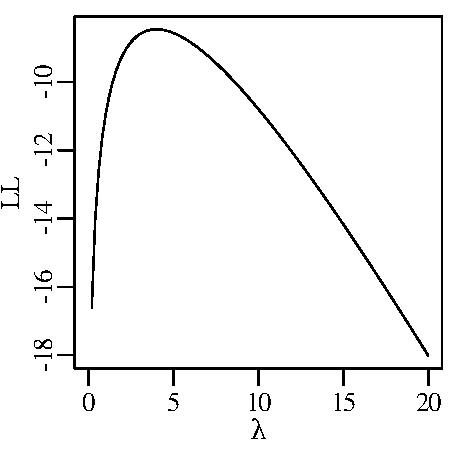
\includegraphics[width=\textwidth]{../figures/LLpois.pdf}\medskip
\end{minipage}
\begin{minipage}[t][][t]{.7\linewidth}
  \captionof{figure}{Log-likelihood function for the Poisson
    distribution, evaluated at different values for the parameter
    $\lambda$, given an observation of $k=4$ successes. The function
    reaches a maximum value at $\hat{\lambda}=4$.  }
  \label{fig:LLpois}
\end{minipage}

\item We can find the maximum likelihood estimate for $\lambda$ using
  \texttt{R}'s general purpose \texttt{optim} function\footnote{An
    alternative (and easier) function is \texttt{optimise} but this
    does not compute the Hessian matrix.}, using \texttt{par=1} as an
  initial guess for $\lambda$:

\begin{script}[firstnumber=11]
o <-  optim(par=1,f=LL,k=4,control=list(fnscale=-1),method='BFGS')
\end{script}

The control parameter \texttt{fnscale=-1} ensures that \texttt{optim}
finds the \textit{maximum} value of \texttt{LL} rather than its
minimum (which is the default).  And \texttt{BFGS} is one of several
minimisation algorithms that is well suited for one-dimensional
optimisation problems. See \texttt{?optim} for further details.  The
maximum likelihood estimate is then obtained by:

\begin{console}
> o$par
[1] 4.000001
\end{console}

\noindent which yields a value of $\hat{\lambda}=4$, ignoring a small
numerical error.

\item To estimate the uncertainty of $\hat{\lambda}$ using the Fisher
  Information approach of Equation~\ref{eq:Fisher} requires just a
  small change to our code:

\begin{script}[firstnumber=11]
o <-  optim(par=1,f=LL,k=4,control=list(fnscale=-1),
            method='BFGS',hessian=TRUE)
\end{script}

Equation~\ref{eq:Fisher} then becomes:

\begin{console}
> -1/o$hessian
         [,1]
[1,] 4.000001
\end{console}

So $s[\hat{\lambda}]^2=4$, which is the same result as we derived by
hand in Equation~\ref{eq:poisvar}.

\end{enumerate}

\section{Comparing distributions}
\label{sec:R-comparingdistributions}

\begin{enumerate}

\item Create a Q-Q plot comparing the Old Faithful eruption durations
  with the eruption waiting times:

\begin{script}
qqplot(faithful[,'eruptions'],faithful[,'waiting'])
\end{script}

Create a Q-Q plot comparing the eruption durations with a normal
distribution (Figure~\ref{fig:qqfaithful1}):

\begin{script}
dat <- faithful[,'eruptions']
qqnorm(dat)
qqline(dat)
\end{script}

\item Perform the one-sided, one-sample t-test of Section~\ref{sec:t}
  (page~\pageref{eq:t}):

\begin{script}
gold1 <- c(19.09,19.17,19.31,19.07,19.18)
h <- t.test(x=gold1,mu=19.30,alternative='less')
\end{script}

The p-value of this test is

\begin{console}
> h$p.value
[1] 0.01630814
\end{console}

\noindent which is less than 0.05, leading to a rejection of $H_0: \mu=19.30$.
Equivalently, the 95\% confidence interval is

\begin{console}
> h$conf.int
[1]     -Inf 19.25435
\end{console}

$\mu=19.30\notin(-\infty,19.25435]$, which again leads to a rejected
null hypothesis.

\item\label{it:2sided2samplettest} Comparing two sets of coins with a
  two-sided, two-sample test:

\begin{script}[firstnumber=2]
gold2 <- c(19.30,19.33,19.15,19.32)
h <- t.test(x=gold1,y=gold2,var.equal=TRUE)
\end{script}

Inspecting the p-value and two-sided 95\% confidence interval:

\begin{console}
> h$p.value
[1] 0.1099177
> h$conf.int
[1] -0.25441458  0.03241458
\end{console}

We cannot reject $H_0: \mu_1=\mu_2$ because $0.1099177>0.05$, and
because $\{-0.25441458\leq{0}\leq{0.03241458}\}$.

\item To carry out the $\chi^2$-test of Section~\ref{sec:contingency},
  we simply supply a contingency table of petrographic observations to
  the \texttt{chisq.test()} function:

\begin{script}
petrography <- rbind(sampleA=c(Q=10,P=5,A=6,L=20),
                     sampleB=c(Q=25,P=12,A=10,L=35))
h <- chisq.test(x=petrography)
\end{script}

\noindent where \texttt{rbind} binds the two named rows together into
one matrix. Querying the results of the test at the console:

\begin{console}
> h
	Pearson's Chi-squared test

data:  petrography
X-squared = 0.82706, df = 3, p-value = 0.843
\end{console}

$0.843>0.05$, hence $H_0$ is not rejected. Note that the
$\chi^2$-statistic is not exactly the same as value that was
calculated by hand in Section~\ref{sec:contingency}. This is due to
rounding errors of the expected counts ($E_i$ in
Equation~\ref{eq:chi2}). Here are the exact values:

\begin{console}
> h$expected
               Q         P         A        L
sampleA 11.66667  5.666667  5.333333 18.33333
sampleB 23.33333 11.333333 10.666667 36.66667
\end{console}

\item Comparing the two collections of gold coins from
  item~\ref{it:2sided2samplettest} above but this time using a
  Wilcoxon test instead of a t-test:

\begin{script}
gold1 <- c(19.09,19.17,19.31,19.07,19.18)
gold2 <- c(19.30,19.33,19.15,19.32)
h <- wilcox.test(x=gold1,y=gold2)
\end{script}

Querying the p-value:

\begin{console}
> h$p.value
[1] 0.1904762
\end{console}

We cannot reject $H_0$ because $0.1904762>0.05$.

\item Extract two detrital zircon U--Pb age distributions for the Mu
  Us desert and Yellow River from \texttt{geostats}' built-in
  \texttt{DZ} dataset, and compare them with the Kolmogorov-Smirnov
  test:

\begin{script}
river <- DZ[['Y']]
dune <- DZ[['5']]
h <- ks.test(x=river,y=dune)
\end{script}

Querying the result:

\begin{console}
> h$p.value
[1] 4.500822e-05
\end{console}

$4.500822\times{10}^{-5}\ll{0.05}$ and hence $H_0$ is clearly rejected.

\end{enumerate}

\section{Regression}
\label{sec:R-regression}

\begin{enumerate}

\item \texttt{geostats} contains a Rb--Sr dataset called
  \texttt{rbsr}.  Plot the columns \texttt{RbSr} and \texttt{SrSr} of
  this dataset as a scatter plot:

\begin{script}
plot(x=rbsr$RbSr,y=rbsr$SrSr)
\end{script}

Calculate the correlation coefficient of \texttt{RbSr} and
\texttt{SrSr}:

\begin{script}[firstnumber=2]
r <- cor(x=rbsr$RbSr,y=rbsr$SrSr)
\end{script}

\noindent which yields:

\begin{console}
> r
[1] 0.9847415
> r^2
[1] 0.9697158
\end{console}

\item Compute the t-statistic for the correlation coefficient using
  Equation~\ref{eq:tr}:

\begin{script}[firstnumber=3]
n <- nrow(rbsr)
tstat <- r*sqrt(n-2)/sqrt(1-r^2)
\end{script}

\noindent Query the value at the console and compare it to the
rejection region for a two-sided t-test:

\begin{console}
> tstat
[1] 13.86085
> qt(c(0.025,0.975),df=n-2)
[1] -2.446912  2.446912
\end{console}

\noindent The observed value for the t-statistic falls in the
rejection region ($13.86085 > 2.446912$). Thus $H_0$ is rejected and
the linear trend is real. Alternatively, we can also perform the
correlation test using \texttt{R}'s \texttt{cor.test()} function:

\begin{console}
> h <- cor.test(x=rbsr$RbSr,y=rbsr$SrSr)
> h$p.value
[1] 8.779983e-06
\end{console}

\noindent which is less than $\alpha=0.05$, again leading to the
rejection of $H_0$.

\item Having demonstrated the statistical significance of the
  correlation, we can now fit a line to the data using the method of
  least squares:

\begin{script}[firstnumber=2]
fit <- lm(SrSr ~ RbSr, data=rbsr)
\end{script}

\noindent which uses \texttt{R}'s \textbf{formula notation}
(\verb|Y ~ X| where \texttt{X} is the independent variable and
\texttt{Y} is the dependent variable)\footnote{Many other \texttt{R}
  functions also accept formula notation, e.g. \texttt{plot(SrSr
    \textasciitilde{} RbSr, data=rbsr)}}.

The output of \texttt{lm()} can be queried like a list to retrieve the
slope and intercept:

\begin{console}
> fit$coefficients
(Intercept)        RbSr 
 0.69742660  0.01391808
\end{console}

The best fit line is given by
[\textsuperscript{87}Sr/\textsuperscript{86}Sr] = 0.696 + 0.014
[\textsuperscript{87}Rb/\textsuperscript{86}Sr] (rounded to two
significant digits).

\item Predict the \textsuperscript{87}Sr/\textsuperscript{86}Sr-value
  for \textsuperscript{87}Rb/\textsuperscript{86}Sr = 10, say:
  
\begin{console}
> fit$coefficients[1] + fit$coefficients[2]*10
(Intercept)
  0.8366074 
\end{console}

Equivalently:

\begin{console}
> predict(fit, newdata=data.frame(RbSr=10))
        1 
0.8366074
\end{console}

\item Add the best fit line to the existing scatter plot:

\begin{script}[firstnumber=3]
abline(fit)
\end{script}

Construct a 95\% confidence envelope for the linear fit:

\begin{script}[firstnumber=4]
x <- seq(from=min(rbsr$RbSr),to=max(rbsr$RbSr),length.out=20)
pred <- predict(fit,newdata=data.frame(RbSr=x),
                interval="confidence",level=0.95)
matlines(x,pred,lty=1,col='black')
\end{script}

\noindent where \texttt{matlines} simultaneously plots multiple lines.
Adding a prediction interval to the existing plot:

\begin{script}[firstnumber=8]
pred <- predict(fit,newdata=data.frame(RbSr=x),
                interval="prediction",level=0.95)
matlines(x,pred,lty=2,col='black')
\end{script}

\item The \texttt{rbsr} file contains five columns, specifying the
  ratios as well as their uncertainties and error correlations:

\begin{console}
> rbsr
  RbSr errRbSr  SrSr errSrSr   rho
1 2.90  0.0944 0.745 0.00702 0.586
2 7.14  0.0970 0.803 0.00625 0.470
3 9.10  0.1040 0.823 0.00740 0.476
4 3.41  0.1040 0.737 0.00697 0.468
5 1.91  0.0967 0.720 0.00676 0.486
6 7.15  0.1110 0.793 0.00749 0.507
7 5.92  0.0948 0.789 0.00632 0.561
8 8.28  0.1070 0.807 0.00678 0.460
\end{console}

Plotting these data as error ellipses and implementing the
weighted least squares regression algorithm of
Section~\ref{sec:weightedregression} is not trivial in base
\texttt{R}. Fortunately, the \texttt{geostats} package comes to the
rescue:

\begin{script}
yfit <- york(dat=rbsr)
\end{script}

The name of the weighted least squares regression refers to
geophysicist Derek York, who developed an early version of the
algorithm\footnote{York, D., 1968. Least squares fitting of a straight
  line with correlated errors. \emph{Earth and Planetary Science
    Letters}, 5, pp.320-324.}.

\end{enumerate}

\section{Fractals and chaos}
\label{sec:R-fractals}

\begin{enumerate}
  
\item\label{it:finland} Calculate and plot the size-frequency
  distribution of Finnish lakes (Figure~\ref{fig:Finlandpowerlaw}):

\begin{script}
sf <- sizefrequency(Finland$area)
plot(frequency~size,data=sf,log='xy')
fit <- lm(log(frequency)~log(size),data=sf)
lines(x=sf$size,y=exp(predict(fit)))
\end{script}

\noindent where the \texttt{sizefrequency()} function is provided by
\texttt{geostats}.\medskip

\item Create a Gutenberg-Richter plot for the recent earthquake data
  (Figure~\ref{fig:gutenberg}):

\begin{script}
gutenberg(earthquakes$mag)
\end{script}

\noindent where \texttt{gutenberg()} is a \texttt{geostats} function
that is similar to the Finnish lake code of step~\ref{it:finland}. You
can check out the implementation details by typing
`\texttt{gutenberg}' at the command prompt.

\item Create a \textit{Koch snowflake}, i.e. a triangle of three Koch
  curves (Figures~\ref{fig:koch1}-\ref{fig:koch6}):

\begin{script}
k <- koch(n=5)
\end{script}

Compute the fractal dimension of the curve:

\begin{script}[firstnumber=2]
fit <- fractaldim(k)
\end{script}

\noindent which yield a slope of -1.2 and, hence, a fractal dimension
of 1.2.

\end{enumerate}

\section{Unsupervised learning}
\label{sec:R-unsupervised}

\begin{enumerate}

\item The \texttt{geostats} package includes a function called
  \texttt{PCA2D()} that can be used to reproduce
  Figures~\ref{fig:PCA2D1}--\ref{fig:PCA2D3}:

\begin{script}
X <- rbind(c(-1,7),c(3,2),c(4,3))
colnames(X) <- c('a','b')
PCA2D(X)
\end{script}

\item Verifying the equivalence of PCA and classical MDS:

\begin{script}[firstnumber=3]
d <- dist(X)           # create a Euclidean distance matrix
conf <- cmdscale(d)    # classical MDS
plot(conf,type='n')    # create an empty plot
text(conf,labels=1:3)  # add text labels to the empty plot
\end{script}

This script produces the same output as the first panel of
\texttt{PCA2D}.

\item \texttt{R} contains not one but two built-in PCA functions:
  \texttt{prcomp} and \texttt{princomp}. Both produce essentially the
  same output but use different algebraic
  algorithms\footnote{\texttt{prcomp} uses singular value
  decomposition, whereas \texttt{princomp} uses an eigen
  decomposition.}. Applying \texttt{prcomp} to the US arrests data to
  produce the biplot shown in Figure~\ref{fig:USArrests}:

\begin{script}
pc <- prcomp(USArrests,scale.=TRUE)
biplot(pc)
\end{script}

\item Reproducing the MDS analysis of European road distances of
  Figure~\ref{fig:eurodist}:

\begin{script}
conf <- cmdscale(eurodist)
plot(conf,type='n',asp=1)
text(conf,labels=labels(eurodist))
\end{script}

Repeating the same exercise using nonmetric MDS:

\begin{script}
library(MASS)
mds <- isoMDS(eurodist)
conf <- mds$points
plot(conf,type='n',asp=1)
text(conf,labels=labels(eurodist))
\end{script}

Flip the y-axis to make the MDS configuration look more like the map
of Europe:

\begin{script}[firstnumber=4]
ylim <- rev(range(conf[,2])) # reverse the minimum and maximum values
plot(conf,type='n',asp=1,ylim=ylim) # change the y-axis limits
\end{script}

Assess the goodness of fit on a Shepard plot:

\begin{script}[firstnumber=4]
sh <- Shepard(d=eurodist,x=conf)  
stress <- signif(mds$stress,2)
plot(sh,main=paste0('stress=',stress))
\end{script}

\noindent where \texttt{signif(x,2)} rounds \texttt{x} to 2
significant digits.

\item\label{it:R-kmeans} Visualise the iris data in a ${4}\times{4}$
  grid of scatter plots (Figure~\ref{fig:Iris}):

\begin{script}
measurements <- iris[,-5]
species <- iris[,5]
plot(measurements,pch=as.numeric(species))
\end{script}

\noindent where \texttt{as.numeric} converts the species to numbers,
which are subsequently used as colours. Classify the data into three
groups using the k-means algorithm:

\begin{script}[firstnumber=4]
fit <- kmeans(measurements,centers=3)
\end{script}

Compare the classes to the known species of the flowers:

\begin{console}
> table(fit$cluster,species)
    setosa versicolor virginica
  1      0          2        36
  2      0         48        14
  3     50          0         0
\end{console}

\item Hierarchical clustering of the iris data:

\begin{script}
tree <- hclust(dist(measurements))
plot(tree)
\end{script}

Cutting the tree down to three branches:

\begin{script}
treecut <- cutree(tree,k=3)
table(treecut,species)
\end{script}

\end{enumerate}

\section{Supervised learning}
\label{sec:R-supervised}

\begin{enumerate}
\item\label{it:LDA} Discriminant analysis is implemented in the
  \texttt{MASS} package:

\begin{script}
library(MASS)
ld <- lda(Species ~ ., data=iris)
\end{script}

Predict the species of a new flower with a sepal length of 6.0~cm, a
sepal width of 3.0~cm, a petal length of 5.0~cm and a petal width of
1.5~cm:

\begin{script}[firstnumber=3]
newflower <- data.frame(Sepal.Length=6.0,Sepal.Width=3.0,
                        Petal.Length=5.0,Petal.Width=1.5)
pred <- predict(ld,newdata=newflower)
\end{script}

Query the posterior likelihoods of the LDA classification:

\begin{console}
> pred$posterior
        setosa versicolor virginica
1 3.207192e-27  0.8098087 0.1901913
\end{console}

\noindent which means that there is an 81\% chance that the new flower
is \textit{versicolor} and a 19\% chance that it is
\textit{virginica}.

Hence the predicted species of the new flower is:

\begin{console}
> pred$class
[1] versicolor
\end{console}

\item To apply quadratic discriminant analysis, we simply replace
  \texttt{lda} by \texttt{qda} in the previous code:

\begin{script}[firstnumber=2]
qd <- qda(Species ~ ., data=iris)
\end{script}

\noindent which produces the following outcome:

\begin{console}
> predict(qd,newdata=newflower)$posterior
         setosa versicolor virginica
1 2.147589e-103  0.7583223 0.2416777
\end{console}

Thus, according to QDA, there is a 76\% probability that the new
flower is \textit{versicolor}, and a 24\% chance that it is
\textit{virginica}.

\item Decision trees are implemented in the \texttt{rpart} package:

\begin{script}
library(rpart)
tree <- rpart(Species ~ ., data=iris, method="class")
plot(tree)
text(tree)
\end{script}

To add the misclassification rates to the tree:

\begin{script}[firstnumber=4]
text(tree, use.n=TRUE)
\end{script}

Using the \texttt{newflower} data frame that we created in
step~\ref{it:LDA}, the class probabilities are:

\begin{console}
> predict(object=tree,newdata=newflower)
  setosa versicolor  virginica
1      0  0.9074074 0.09259259
\end{console}

\noindent which leads to the following classification:

\begin{console}
> predict(object=tree,newdata=newflower,type='class')
         1 
versicolor 
\end{console}

\end{enumerate}
  
\section{Compositional data}
\label{sec:R-compositional}

\begin{enumerate}

\item Transform the A--CN--K data of Section~\ref{sec:logratios} from
  the ternary simplex to bivariate logratio space using the alr
  transformation:

\begin{script}
uv <- alr(ACNK)
plot(uv)
\end{script}

\noindent where the \texttt{alr()} function is provided by the
\texttt{geostats} package (type \texttt{alr} at the command prompt to
see the code). Computing the mean and covariance matrix of the
logratio data:

\begin{script}[firstnumber=3]
mu <- colMeans(uv)
covmat <- cov(uv)
\end{script}

Add the mean to the logratio plot as a black square and the confidence
ellipse as a polygon:

\begin{script}[firstnumber=5]
points(x=mu[1],y=mu[2],pch=22,bg='black')
ell <- ellipse(mu,covmat)
polygon(ell)
\end{script}

\item Plot the A--CN--K data on a ternary diagram:

\begin{script}
ternary(ACNK,labels=c(expression('Al'[2]*'O'[3]),
                      expression('CaO+Na'[2]*'O'),
                      expression('K'[2]*'O')))
\end{script}

\noindent where the \texttt{expression} function allows \texttt{R} to
use subscripts and special characters in text labels. Mapping the
logratio mean and error ellipse back to the ternary diagram:

\begin{script}[firstnumber=4]
ternary(alr(mu,inverse=TRUE),add=TRUE,type='p',pch=22,bg='black')
ternary(alr(ell,inverse=TRUE),add=TRUE,type='l')
\end{script}

\item Apply PCA to the major element compositions of
  Table~\ref{tab:Major}:

\begin{script}
comp <- clr(major)
pc <- prcomp(comp)
biplot(pc)
\end{script}

\item Apply LDA to the AFM data of Figure~\ref{fig:AFM}:

\begin{script}
library(MASS)
affinity <- FAM[,1]
comp <- alr(FAM[,-1])
ld <- lda(x=comp,grouping=affinity)
\end{script}

\noindent where the \texttt{lda} function does not use formula
notation (Section~\ref{sec:R-supervised}) but an alternative format
(see \texttt{?lda} for further details).  Classify a new rock with
1~wt\% FeO, 8~wt\% Na\textsubscript{2}O+K\textsubscript{2}O, and
0.1~wt\% MgO:

\begin{script}[firstnumber=5]
newrock <- data.frame(F=1,A=8,M=0.1)
newcomp <- alr(newrock)
pr <- predict(object=ld,newdata=newcomp)
\end{script}

This produces:

\begin{console}
> pr$posterior
            ca          th
[1,] 0.9931941 0.006805909
\end{console}

\noindent which suggests that the new sample is a calc-alkaline
basalt.

\end{enumerate}

\section{Directional data}
\label{sec:R-directional}

Base \texttt{R} includes little or no functionality for directional
data analysis. So this tutorial will heavily depend on the
\texttt{geostats} package.

\begin{enumerate}

\item Plot the glacial striations data on a circle:

\begin{script}
circle.plot(striations,degrees=TRUE)
\end{script}

\noindent where the \texttt{degrees} option accounts for the fact that
the \texttt{striations} data are expressed in degrees.  Change to
\texttt{degrees=FALSE} for radians. Add the arithmetic mean and vector
mean to the plot as a white and black square, respectively:

\begin{script}[firstnumber=2]
circle.points(mean(striations),pch=22,bg='white',degrees=TRUE)
md <- meanangle(striations,degrees=TRUE)
circle.points(md,pch=21,bg='black',degrees=TRUE)
\end{script}

\item\label{it:Rbar} Compute the concentration parameter $\bar{R}$:

\begin{script}
R <- Rbar(striations,degrees=TRUE)
\end{script}

Converting to the von Mises parameter $\kappa$ using
Equation~\ref{eq:kappa}:

\begin{script}[firstnumber=2]
k <- Rbar2kappa(R)
\end{script}

Evaluating the von Mises distribution over the 0 -- 360$^{\circ}$
interval:

\begin{script}[firstnumber=3]
a <- seq(from=0,to=360,length.out=100)
d <- vonMises(a,mu=md,kappa=k,degrees=TRUE)
plot(a,d,type='l')
rug(striations)
\end{script}

\item To plot azimuths and dips on a Wulff stereonet:

\begin{script}
stereonet(trd=palaeomag$decl,plg=palaeomag$incl,
          option=1,degrees=TRUE,show.grid=FALSE)
\end{script}

For strikes and dips, use the \texttt{option=2} argument:

\begin{script}
stereonet(trd=fault$strike,plg=fault$dip,
          option=2,degrees=TRUE,show.grid=FALSE)
\end{script}

To plot geographical coordinates (e.g, 30$^\circ$ longitude and
-20$^\circ$ latitude) on a Schmidt stereonet:

\begin{script}
stereonet(trd=30,plg=-20,degrees=TRUE,
          option=3,show.grid=TRUE,wulff=FALSE)
\end{script}

To add five cones of 10 degree radius to the existing plot (as in
Figure~\ref{fig:wulffschmidt}.b):

\begin{script}[firstnumber=3]
stereonet(trd=c(0,0,90,180,270),plg=c(90,10,10,10,10),
          coneAngle=rep(10,5),option=4,degrees=TRUE,add=TRUE,wulff=FALSE)
\end{script}

\item To compute the average azimuth and dip and add it to a Wulff net:

\begin{script}
A <- palaeomag$decl
D <- palaeomag$incl
meanpalaeomag <- meanangle(trd=A,plg=D,option=1,degrees=TRUE)
stereonet(trd=A,plg=D,degrees=TRUE,show.grid=FALSE,pch=16,col='grey')
stereonet(trd=meanpalaeomag[1],plg=meanpalaeomag[2],
          option=1,degrees=TRUE,add=TRUE,pch=16,col='black')
\end{script}

To average strike and dip measurements:

\begin{script}
S <- fault$strike
D <- fault$dip
meanfault <- meanangle(trd=S,plg=D,option=2,degrees=TRUE)
stereonet(trd=S,plg=D,option=2,degrees=TRUE,
          show.grid=FALSE,pch=16,col='grey')
stereonet(trd=meanfault[1],plg=meanfault[2],
          option=2,degrees=TRUE,add=TRUE,pch=16,col='black')
\end{script}

\item To compute the average orientation of the pebble measurements:

\begin{script}
circle.plot(pebbles,degrees=TRUE)
m <- meanangle(pebbles,degrees=TRUE,orientation=TRUE)
circle.points(m,degrees=TRUE,pch=16,cex=2)
\end{script}  

\end{enumerate}

\section{Spatial data}
\label{sec:R-spatial}

\texttt{geostats} implements a simple version of ordinary kriging.  A
far more complete set of geostatistical functions can be found in the
\texttt{gstat} package.

\begin{enumerate}

\item Load the Meuse dataset, define three shorthand variables, and
  plot them on a map:

\begin{script}
X <- meuse$x  # Easting
Y <- meuse$y  # Northing
Z <- log(meuse$zinc)
colourplot(X=X,Y=Y,Z=Z,key.title=title('ln[Zn]'))
\end{script}

\item Plot the empirical semivariogram and fit a spherical
  semivariogram model to it:

\begin{script}[firstnumber=4]
svm <- semivariogram(x=X,y=Y,z=Z)
\end{script}

Query the fit parameters:

\begin{console}
> svm$snr
        sill       nugget        range 
  0.63756843   0.03512741 892.01855323 
\end{console}

To fit an exponential semivariogram model:

\begin{script}[firstnumber=4]
svm_exp <- semivariogram(x=X,y=Y,z=Z,model='exponential')
\end{script}

The third option for the \texttt{model} argument is \verb|'gaussian'|.

\item Estimating the ln[Zn]-value for the new location
  $\{x_\circ=179850,y_\circ=331650\}$:

\begin{console}
> kriging(x=X,y=Y,z=Z,svm=svm,xi=179850,yi=331650)
[1] 5.011715
\end{console}

\noindent and its variance:

\begin{console}
> kriging(x=X,y=Y,z=Z,svm=svm,xi=179850,yi=331650,err=TRUE)
[1] 0.2215261
\end{console}

\item\label{it:R-meuse-contour} Evaluate the ln[Zn]-values for a grid
  of locations and plot as a contour map:

\begin{script}[firstnumber=5]
xi <- seq(from=min(X),to=max(X),length.out=50)
yi <- seq(from=min(Y),to=max(Y),length.out=50)
zi <- kriging(x=X,y=Y,z=Z,svm=svm,xi=xi,yi=yi,grid=TRUE)
colourplot(x=xi,y=yi,z=zi,key.title=title('ln[Zn]'))
\end{script}

And to visualise the uncertainties of the kriging estimates,
replace the last two lines with:

\begin{script}[firstnumber=7]
zi <- kriging(x=X,y=Y,z=Z,svm=svm,xi=xi,yi=yi,grid=TRUE,err=TRUE)
colourplot(x=xi,y=yi,z=sqrt(zi),key.title=title('s[Zn]/Zn'))
\end{script}

\end{enumerate}
